\documentclass[12pt,a4paper]{article}  % Déclare la classe du document.

\newcommand{\chaptermark}[2]{\og #2 \fg{} (#1)} % ligne uniquement pour éviter une erreur en cas d'article
\include{../1ere-preambule}
\usepackage{mathrsfs}

\usepackage{epic}   % extension et simplification de  l'environnement picture
\usepackage{graphicx}    % permet d'inclure des graphique externe dans un document
\usepackage{arydshln}   %permet d'avoir des lignes en pointillés

\newcommand{\lignes}[1]{
\setlength{\unitlength}{1mm}
\vskip 0,4cm\noindent
\multido{\i=0+1}{#1}{%
     \noindent
     \begin{picture}(150,5)
     \linethickness{0,005mm}
     \put(-5,0){\dashline{1}(175,5)(5,5)}
     \end{picture}\vskip 0,001cm
     }
\vskip 0cm
}

\rhead{\textcolor{red}{Correction - DS n$^{\circ}$03 - 18/01/2023}}

\begin{document}

\begin{center}
\fbox{
\begin{minipage}[]{15cm}
\begin{center}
\LARGE{\rule{0.5cm}{0pt}\rule[-0.25cm]{0pt}{0.9cm}
\textcolor{red}{Correction -DS n$^{\circ}$3\\
Équations du second degré}\\
}
\end{center}
\end{minipage}
}

\end{center}


%\begin{center}\textbf{2 heures - Calculatrice autorisée - Barème indicatif}\end{center}
%
%%\begin{center}\textbf{Les élèves avec un tier-temps ne traitent pas les questions avec  le symbole \ding{46}}\end{center}
%
%\begin{center}
%%On veillera à ENCADRER ses résultats et soigner sa copie.\\
%Les résultats doivent être justifiés par des calculs (au moins 1 étape intermédiaire).
%\end{center}
\vspace{.05cm} 

\vspace*{-0.5cm}
\exerciceDS{ - Equations - ( 3 points )}

Déterminer les racines des fonctions polynômes du second degré.
\begin{multicols}{2}
\begin{enumMet}
    \item $f(x)=3(x+7)(-x+11)$ \bareme{1}\\
    \begin{corrBox}
    	$x+7=0$ et $-x+11=0$\\
    	$\iff x_1=-7$ et $x_2=11$
    \end{corrBox}
    \item $g(x)=x(x-45)$ \bareme{1}\\
    \begin{corrBox}
    	$x=0$ et $x-45=0$\\
    	$\iff x_1=0$ et $x_2=45$
    \end{corrBox}
	\columnbreak
    \item $h(x)=-4(x+6)(x-501)$ \bareme{1}\\
    \begin{corrBox}
    	$ x+6=0$ et $x-501=0$\\
    	$\iff x_1=-6$ et $x_2=501$
    \end{corrBox}
\end{enumMet}
\end{multicols}

\vspace{-0.3cm}
\exerciceDS{ - Factorisation - ( 6 points )}

Donner les racines du polynôme du second degré donné, puis le factoriser
\begin{multicols}{2}
\begin{enumMet}
    \item $A(x)=x^{2}+6 x+9$ \bareme{1,5}
    \begin{corrBox}
    	$A(x)=x^{2}+6 x+9=(x+3)^2$\\
    	(Identité remarquable)
    \end{corrBox}
    \item $B(x)=\dfrac{2}{3}x^{2}-\dfrac{5}{7} x-\dfrac{3}{7}$ \bareme{1,5}
    \begin{corrBox}
    	$\Delta=b^2-4ac=(-\dfrac{5}{7})^2-4\times\dfrac{2}{3}\times(-\dfrac{3}{7})=\dfrac{81}{49}$\\
    	$x_1=\dfrac{\dfrac{5}{7}-\sqrt{\dfrac{81}{49}}}{2\times\dfrac{2}{3}}=-\dfrac{3}{7}$\\
    	et $x_2=\dfrac{\dfrac{5}{7}+\sqrt{\dfrac{81}{49}}}{2\times\dfrac{2}{3}}=\dfrac{3}{2}$\\
    	$B(x)=\dfrac{2}{3}(x+\dfrac{3}{7})(x-\dfrac{3}{2})$
    \end{corrBox}
	\columnbreak
    \item $C(x)=x^{2}+18 x+77$ \bareme{1,5}
    \begin{corrBox}
    	$C(x)=x^{2}+18 x+77$\\
    	$\Delta=18^2-4\times77=16$\\
    	$x_1=\dfrac{-18-\sqrt{16}}{2}=-11$\\
    	et $x_2=\dfrac{-18+\sqrt{16}}{2}=-7$\\
    	$C(x)=(x+11)(x+7)$
    \end{corrBox}
    \item $D(x)=2 x^{2}-7 x+8$ \bareme{1,5}
    \begin{corrBox}
    	$D(x)=2 x^{2}-7 x+8$\\
    	$\Delta=(-7)^2-4\times2\times8=-15$\\
    	Pas de racines et factorisation impossible.
    \end{corrBox}
\end{enumMet}
\end{multicols}

\vspace{-0.3cm}
\exerciceDS{ - Inéquations - ( 8 points )}

Résoudre les inéquations données.
%\begin{multicols}{2}
\begin{enumMet}
    \item $4 x^{2}-2 x+\dfrac{1}{4}>0$ \bareme{2}
    \begin{corrBox}
    	$\Delta=0$ et $x_0=\dfrac{1}{4}$ et $a>0$ donc\\ $S=\R\textbackslash\left\{\dfrac{1}{4}\right\}$
    \end{corrBox}
    \item $x^{2}-3 x+5 \leqslant 0$ \bareme{2}
    \begin{corrBox}
    	$\Delta=-11$ et $a>0$\\
    	$S=\varnothing$ 
    \end{corrBox}
    \item $6 x^{2}+7 x-3 \geqslant 0$ \bareme{2}
    \begin{corrBox}
    	$\Delta=121$\\
    	$x_1=-\dfrac{3}{2}$\\
    	$x_2=\dfrac{1}{3}$\\
    	\begin{tikzpicture}
    		\tkzTabInit{$x$ / 1 , $f(x)$ / 1}{$-\infty$,$-\dfrac{3}{2}$, $\dfrac{1}{3}$, $+\infty$}
    		\tkzTabLine{, +, z,- , z, +, }
    	\end{tikzpicture}\\
    	$S=\left]-\infty;-\dfrac{3}{2}\right]\cup\left[\dfrac{1}{3}; +\infty\right[$
    \end{corrBox}
    \item $49 x^{2}-4 \geqslant 0$ \bareme{2}
    \begin{corrBox}
    	$\iff (7x-2)(7x+2) \geqslant 0$\\
    	\begin{tikzpicture}
    		\tkzTabInit{$x$ / 1 , $f(x)$ / 1}{$-\infty$,$-\dfrac{2}{7}$, $\dfrac{2}{7}$, $+\infty$}
    		\tkzTabLine{, +, z,- , z, +, }
    	\end{tikzpicture}\\
    	$S=\left]-\infty;-\dfrac{2}{7}\right]\cup\left[\dfrac{2}{7}; +\infty\right[$
    \end{corrBox}
\end{enumMet}
%\end{multicols}

\vspace{-0.3cm}
\exerciceDS{ - Tableau de variations - ( 2 points )}
Pour la fonction polynôme du second degré ci-dessous, dresser son tableau de variations (les valeurs du tableau de variations doivent être justifiées).
$$f(x)=-4x^2+22x+12$$
\begin{corrBox}
	On a $a=-6<0$, $\alpha=-\dfrac{b}{2a}=\dfrac{11}{2}$ et $\beta=f(\alpha)=\dfrac{303}{2}$ donc :\\
	\ \\
	\begin{tikzpicture}
		\tkzTabInit{$x$ / 1 , $f$ / 1.5}{$-\infty$, $\dfrac{11}{2}$, $+\infty$}
		\tkzTabVar{-/ , +/ $\dfrac{303}{2}$, -/ }
	\end{tikzpicture}
\end{corrBox}

\vspace{-0.3cm}
\exerciceDS{ - Somme et Produit de racines - ( 3 points )}

Pour chaque équation, déterminer une solution évidente et en déduire l'autre sans calculer le discriminant.
\begin{multicols}{2}
\begin{enumMet}
    \item $3x^2-4x-7=0$ \bareme{1,5}
    \item $-2x^2+14x-20=0$ \bareme{1,5}
\end{enumMet}
\end{multicols}

\begin{corrBox}
	\begin{multicols}{2}
		\begin{enumMet}
			\item $x_1=-1$, d'ou $S=-\dfrac{b}{a}=\dfrac{4}{3}$\\
			$x_2=\dfrac{4}{3}+1=\dfrac{7}{3}$
			\item $x_1=2$, d'ou $S=-\dfrac{b}{a}=7$\\
			$x_2=7-2=5$
		\end{enumMet}
	\end{multicols}
\end{corrBox}

%\newpage

%\exerciceDS{ - Problème - ( 3 points )}
%
%Le sponsor d'une célèbre équipe de football vend des maillots aux couleurs de l'équipe.\\
%
%Il achète ces maillots à son fournisseur au prix de $10$ \EUR{} l'unité. Il en vend 200 unités par jour à $50$ \EUR{} chacune. Au vu des bons résultats de l'équipe au cours de la saison, il souhaite augmenter le prix de ces maillots.\\
%
%Il réalise une étude de marché qui montre que toute augmentation de $1$ \EUR{} fera baisser la vente de deux maillots par jour. On admet que le nombre de maillots achetés au fournisseur est le même que le nombre de maillots vendus, quel que soit le prix.\\
%
%\textbf{Déterminer le nouveau prix que devra fixer le sponsor pour réaliser un bénéfice maximum.}

\exerciceDS{ - Problème - ( 6 points )}
Une entreprise fabrique et [...] du prix unitaire de vente.
\begin{enumMet}
	\item \begin{enumMet}
		\item Lorsque le prix de vente est de 30 \EUR{}, combien l'entreprise vent-elle de pièces et quel est la recette? \bareme{0,5}
		\begin{corrBox}
			Lorsque le prix de vente est de 30 \EUR{}, l'entreprise vend 1000 pièces et sa recette est $R=30\times1000=30000$
		\end{corrBox}
		\item Lorsque le prix de vente est de 29 \EUR{}, combien l'entreprise vent-elle de pièces et quel est la recette? \bareme{0,5}
		\begin{corrBox}
			Lorsque le prix de vente est de 29 \EUR{}, l'entreprise vend 1100 pièces et sa recette est $R=29\times1100=31900$
		\end{corrBox}
		\item Lorsque le prix de vente est de 28 \EUR{}, combien l'entreprise vent-elle de pièces et quel est la recette? \bareme{0,5}
		\begin{corrBox}
			Lorsque le prix de vente est de 28 \EUR{}, l'entreprise vend 1200 pièce et sa recette est $R=28\times1200=33600$
		\end{corrBox}
	\end{enumMet}
	\item Montrer que $R(x)=100(10+x)(30-x)$. \bareme{1,5}
	\begin{corrBox}
		Le prix de vente est $(30-x)$. Le nombre de pièces vendues est $(1000+100x)$. La recette est donc $R(x)=(30-x)(1000+100x)$.\\
		On peut factoriser par $100$ dans la 2ème parenthèse : $R(x)=100(10+x)(30-x)$.
	\end{corrBox}
	\item Développer $R(x)$. \bareme{1}
	\begin{corrBox}
		$R(x)=100(10+x)(30-x)=100\times(300+30x-10x-x^2)=-100x^2+2000x+30000$
	\end{corrBox}
	\item Écrire $R(x)$ sous forme canonique. \bareme{1}
	\begin{corrBox}
		On a $\alpha=-\dfrac{b}{2a}=10$ et $\beta=f(\alpha)=40000$ donc :\\
		$R(x)=-100(x-10)^2+40000$
	\end{corrBox}
	\item Déterminer le prix de vente unitaire que doit fixer l'entreprise pour que le revenu soit maximum. Quel est ce revenu maximum ? \bareme{1}
	\begin{corrBox}
		Comme $R(x)$ est une fonction du second degré avec $a<0$, le maximum est $\beta$ atteint pour $x=\alpha$. L'entreprise doit donc vendre ses pièces à 20 \EUR{} et le revenu sera alors de $40\ 000$ \EUR{}.
	\end{corrBox}
\end{enumMet}


\exerciceDS{ - Lien entre graphique et calcul - ( 3 points )}
On considère les fonctions $f$ et $g$, de courbes représentatives $\mathscr{C}_f$ et $\mathscr{C}_g$, définies sur $\mathbb{R}$ par:
$$
f(x)=2 x^2+2 x-3 \text { et } g(x)=-x^2-x+3
$$

\begin{enumMet}
	\item A l'aide de la calculatrice, tracer les courbes représentatives $\mathscr{C}_f$ et $\mathscr{C}_g$ des fonctions $f$ et $g$. En déduire la position relative des courbes. \bareme{1} %(Pour quels valeurs de $x$, $\mathscr{C}_f$ est au-dessus de $\mathscr{C}_g$).
%	\item On a tracé ci-dessous les courbes $\mathscr{C}_f$ et $\mathscr{C}_g$. Donner, à l'aide du graphique, la position relative des courbes $\mathscr{C}_f$ et $\mathscr{C}_g$
	\begin{corrBox}
		\begin{center}
			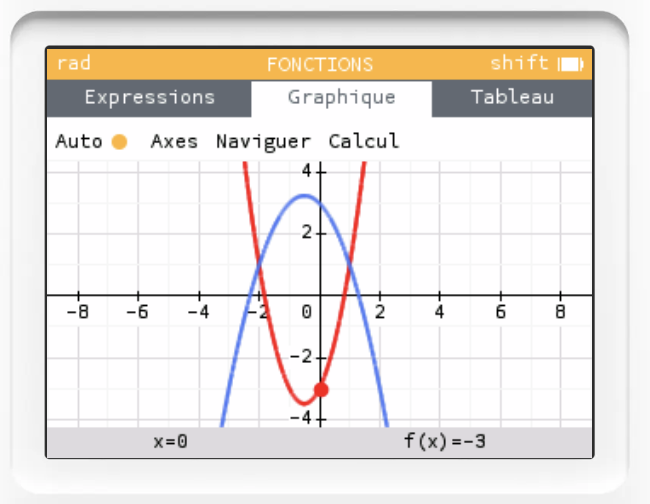
\includegraphics[scale=0.7]{1.03.06-Img01}
		\end{center}
	D'après la calculatrice , la courbe $\mathscr{C}_g$ est au-dessus de la courbe $\mathscr{C}_f$ sur l'intervalle $[-2;1]$.
	\end{corrBox}
	\item Retrouver par le calcul les résultats précédents. \bareme{2}
	\begin{corrBox}
		On étudie le signe de $f(x)-g(x)$\\
		$f(x)-g(x)=2 x^2+2 x-3 -(-x^2-x+3) =3x^2+3x-6$\\
		$x_1=1$ est une racine évidente donc comme $P=-\dfrac{6}{3}=-2$ alors $x_2=-2$\\
		\begin{tikzpicture}
			\tkzTabInit{$x$ / 1 , $f(x)-g(x)$ / 1}{$-\infty$,$-2$, $1$, $+\infty$}
			\tkzTabLine{, +, z,- , z, +, }
		\end{tikzpicture}\\
	$f(x)-g(x)$ est $\leqslant0$ sur $[-2;1]$. On retrouve donc bien le résultat obtenu à l'aide du graphique : a courbe $\mathscr{C}_g$ est au-dessus de la courbe $\mathscr{C}_f$ sur l'intervalle $[-2;1]$.
	\end{corrBox}
\end{enumMet}



\end{document}

